% Chapter 3
\setlength\topmargin{8mm}
\onehalfspacing
\chapter{Disseny} % Main chapter title

\label{Chapter3} % For referencing the chapter elsewhere, use \ref{Chapter1} 

\rhead[\emph{Disseny, programació i implementació d'un robot de dibuix amb Arduino}]{\thepage}
\lhead[\thepage]{\emph{Disseny, programació i implementació d'un robot de dibuix amb Arduino}}

En aquest apartat es descriu el disseny del robot, la creació de l’estructura i la distribució dels components, explicant el perquè d’aquesta distribució i les premisses que s’han tingut en compte a l'hora de dissenyar les diferents peces en Solid Works per tal d'imprimir-les en 3D posteriorment a l'aula Rep Rap de la universitat.   

\begin{figure}[H]
	\centering
	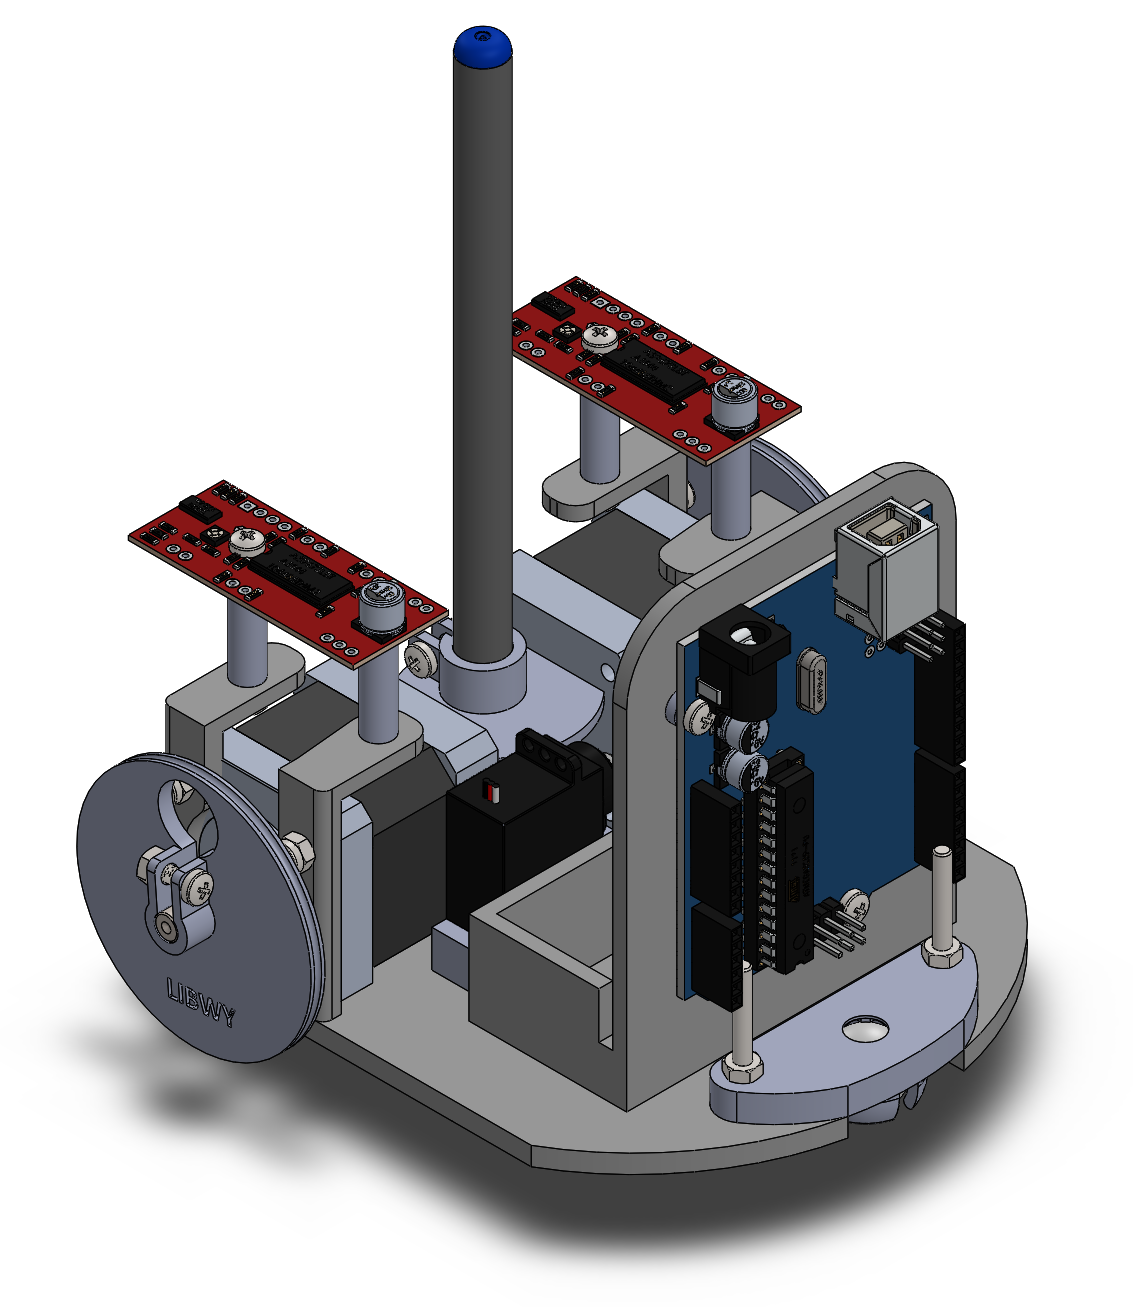
\includegraphics[scale=0.6]{RobotSW.png}
	\caption{Assemblatge del robot en SolidWorks (exceptuant la bateria, el cablejat i el módul Bluetooth).}
	\label{fig:RobotSW}
\end{figure}

\section{Xassís}

El xassís és el cos del robot, incorpora totes les altres peces i el seu disseny és una de les parts fonamentals del treball. És l’encarregat de centrar els eixos dels motors i fixar la seva posició, d’incorporar la bateria, el microcontrolador, els drivers i tot el circuit elèctric, i d'assegurar la seva posició fixa durant el moviment del robot. A continuació es mostra una imatge del disseny del xassís on s'indiquen les parts més importants que després s'explicaran. 

\begin{figure}[H]
	\centering
	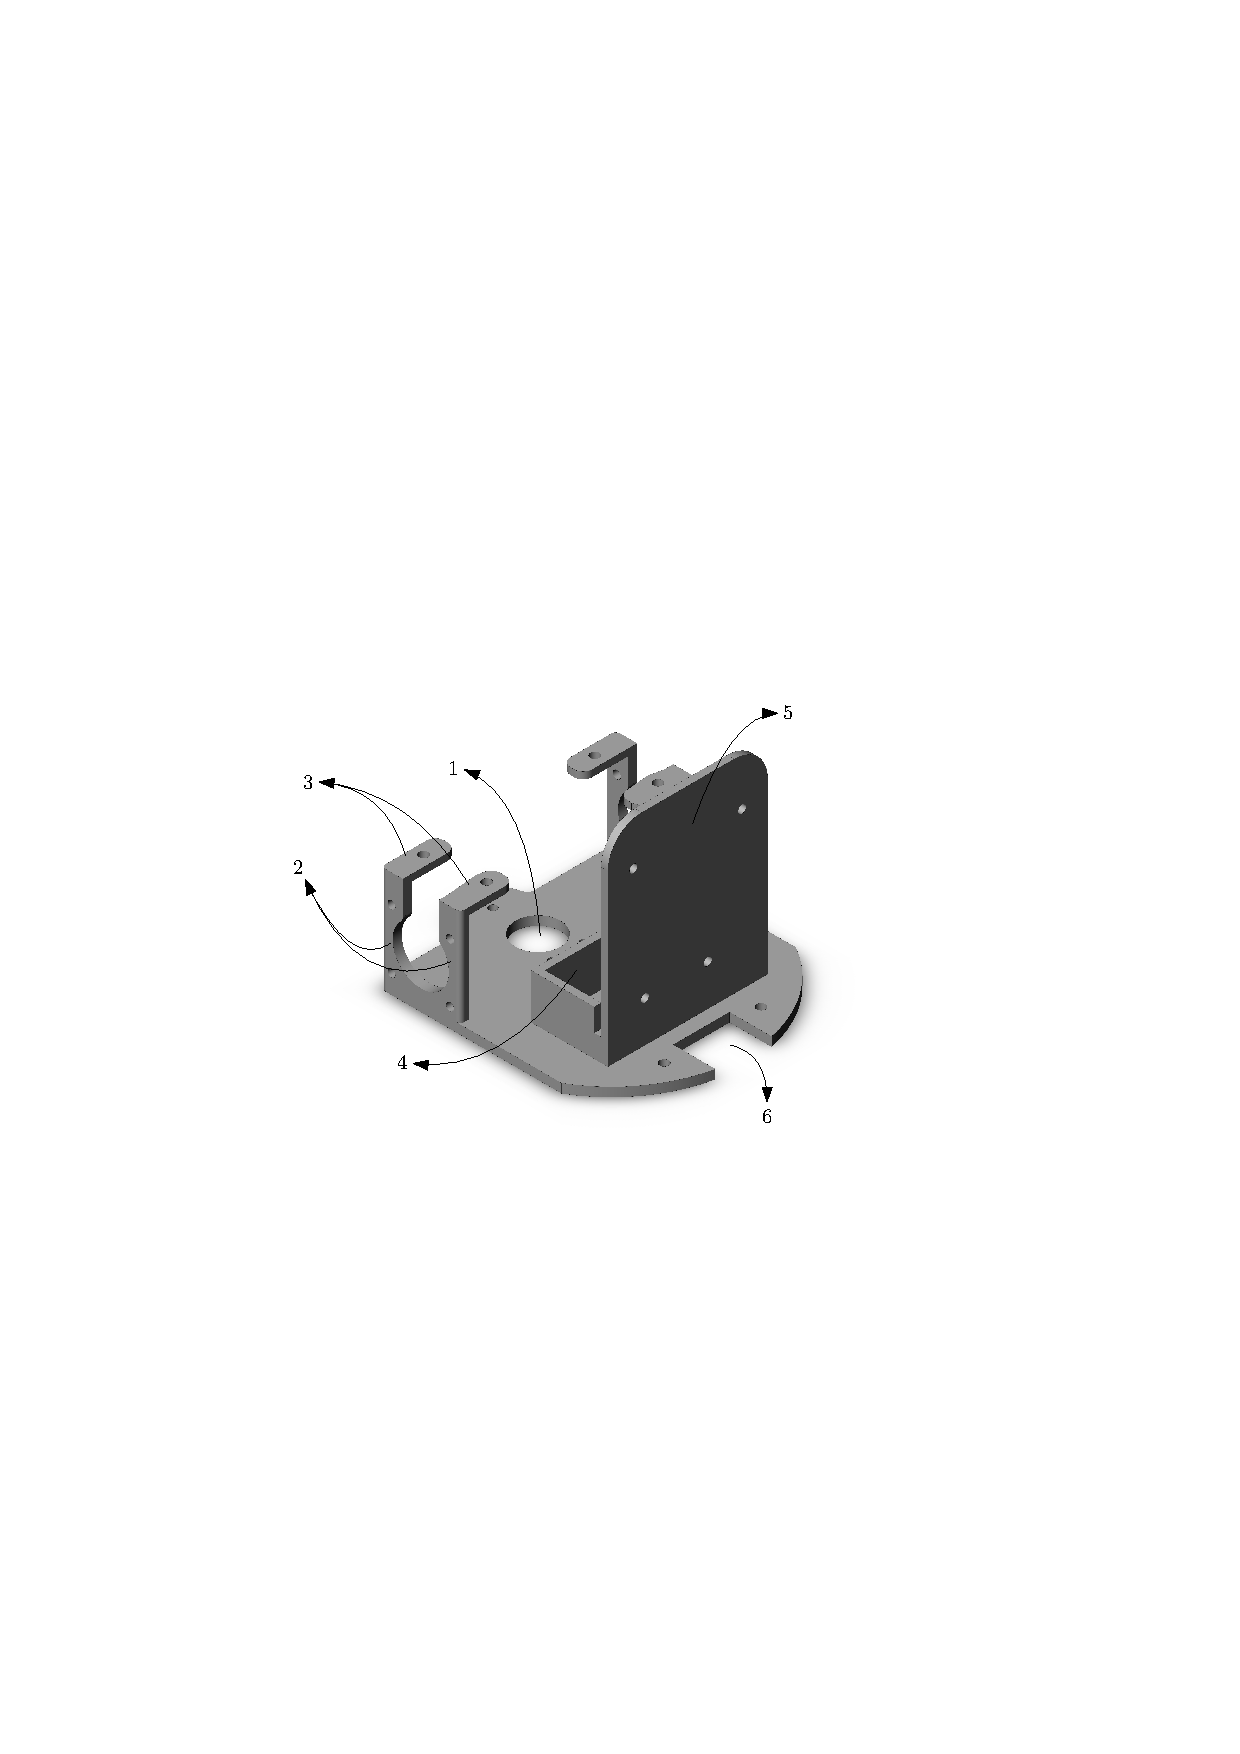
\includegraphics{xassis}
	\caption{Parts del xassís.}
	\label{fig:xassis}
\end{figure}
 
L’objectiu era dissenyar un xassís amb les dimensions més petites possibles, i aquestes van venir donades directament per la mida dels dos motors. S’ha dissenyat  amb una amplada de 104 mm tenint en compte que ha de suportar els dos motors que tenen una llargada de 34 mm i que a l’espai entre els dos cal adaptar el suport del retolador pel qual s'han deixat 28 mm. Els altres 8 mm restants estan reservats per les fixacions dels motors. Per tal de no posar unes limitacions molt restrictives, s’ha decidit realitzar un forat de 20 mm de diàmetre (detall 1 de la imatge \ref{fig:xassis}) per l’element de dibuix, per  adaptar el suport a les mides del retolador o estri escollit. És fonamental que aquest forat estigui centrat entre els dos motors i amb un eix perpendicular i coincident amb els eixos dels motors que han d’estar alineats. D’aquesta manera s’aconsegueix l’amplada mínima, ja que la resta d’elements són de dimensions més reduïdes i ,per tant, s’han posicionat de manera centrada per mantenir centrat el centre de masses. 

Per tal de fixar els motors s’han incorporat uns suports verticals (detall 2) que fixen amb cargols la cara frontal del motor (on neix l’eix) evitant així que pugui desplaçar-se i mantenint d’aquesta manera els dos motors sempre alineats. Aquests suportss es van imprimir incorporats directament al xassís, per minimitzar els possibles errors de muntatge o descentratge. De la mateixa manera, aprofitant aquests suports i per optimitzar l’espai, s’ha incorporat una petita part plana horitzontal (detall 3) sobre els motors per instal·lar-hi els drivers dels mateixos i així mantenir-ho junt i facilitant el reconeixement del driver corresponent a cada motor. Cal destacar que aquests suports no tanquen la part superior de tal manera que es poden muntar i desmuntar els motors de manera més còmoda sense, per exemple, desmuntar el suport del retolador. 

La longitud del xassís ha de ser la suficient per col·locar-hi els motors, el servomotor encarregat d’aixecar el retolador, la bateria, el microcontrolador Arduino i la roda davantera. D’aquesta manera, el xassís final té una llargada de 108,68 mm i la següent distribució: 

En primer lloc es col·loquen els motors de 35 mm d'amplada. Seguidament, hi ha un espai reservat al suport fixe del bolígraf que s’ha dissenyat com una peça diferent per tal de poder adaptar-la a altres utillatges sense haver de modificar el xassís per complet. Disposa d’una base per enganxar el servomotor fixant la seva alçada de manera que l’eix del servo es mantingui a la mateixa alçada que l’extrem del suport fixe, per tal d’exercir la força per aixecar el retolador sobre el suport mòbil des de la posició horitzontal per gaudir del recorregut màxim del moviment si fos necessari. 

En següent lloc, s’ha dissenyat un espai reservat per la bateria (detall 4) que compte amb un petit compartiment que manté la bateria en posició vertical i fixa per evitar que caigui o pugui interrompre el funcionament del robot. Aquest compartiment té una mida de 25 x 65 mm amb tres parets de 20 mm d’alçada i la paret posterior de 90 mm que s’aprofita per fer de base de l’Arduino (detall 5). Es pot observar que les mides són uns mil·límetres més grans que la pròpia bateria, ja que s’ha deixat l’espai suficient per tal de poder posar els cargols per fixar l’Arduino. És per aquesta raó que s’ha deixat un petit espai entre les parets laterals i la paret verical per poder manipular els cargols amb la bateria fixada si fos necessari. S’ha decidit instal·lar la bateria al punt mig del robot per distribuir la massa al llarg del xassís i evitar que el centre de masses quedi a la línia de l’utillatge de dibuix i el robot pugui bolcar en algun punt de la trajectòria degut a algun moviment concret.   

L’Arduino, com s’acaba d’explicar, es col·loca a la paret vertical del compartiment de la bateria de manera que queda fixat verticalment, optimitzant així els espais. S’han dissenyat els forats per tal de col·locar l’entrada del port serial a la part superior fent possible d’aquesta manera la programació de la placa un cop s’ha implementat tot el prototip, ja que sinó s'hauria de desmontar cada cop que es volgués programar. Al lateral de la placa s’han instal·lat dues barres de corrent de protoboard per tal de poder alimentar des de la mateixa sortida de la font un motor conjuntament amb la placa i l’altre motor amb el servomotor. 

Per acabar, a la part davantera s’ha deixat l’espai lliure (detall 6) suficient per instal·lar-hi una roda boja que actuarà com a punt de suport per estabilitzar el robot. S'ha arrodonit la forma davantera per motius completament estètics i s'ha afegit un petit sortint circular a la part posterior (on hi ha els motors) per tal de facilitar la fixació de la guia del retolador.

\section{Guia del retolador} \label{sec:guia}

Aquest suport està dissenyat per funcionar com a guia pel retolador, de manera que el seu desplaçament sigui vertical i centrat per minimitzar l’error de descentratge del mateix. Consta d’una part plana en forma de T i un tub vertical que farà de guia pel retolador. Va fixada al xassís amb 3 cargols. La guia està expressament dissenyat per treballar amb un retolador Edding 1200 (presentat a l’apartat \ref{sec:retolador}) i s’ha dissenyat de manera independent del xassís per així poder fer-la a mida de l’estri que es vulgui utilitzar sense haver de tornar a imprimir tot el cos del robot. 

\begin{figure}[H]
	\centering
	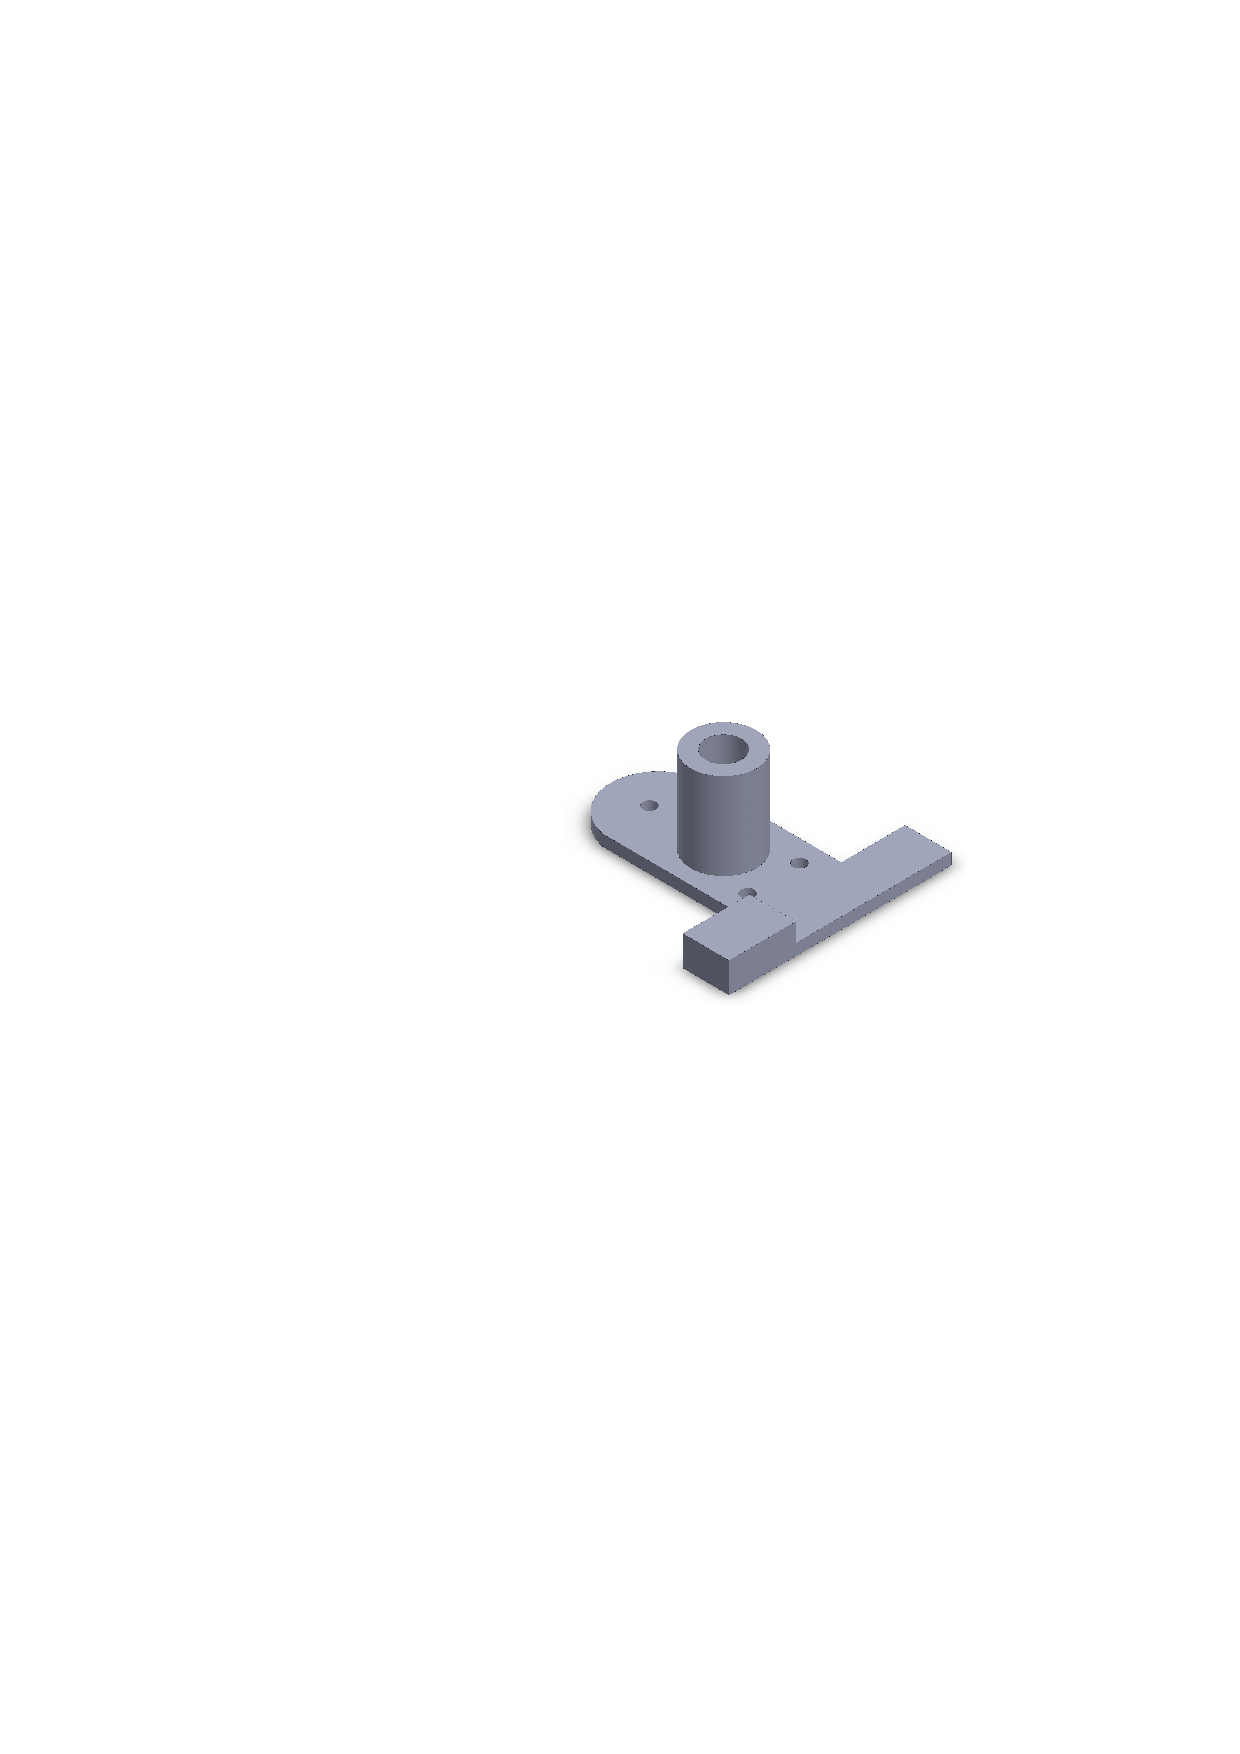
\includegraphics{guia}
	\caption{Imatge del disseny de la guia.}
	\label{fig:guia}
\end{figure}

També compta amb un petit suport per tal d’enganxar el servomotor de manera que l'alçada de l’eix d’aquest sigui lleugerament inferior a l’alçada de la part superior de la guia i aconseguir així que el moviment del servo pugui ser màxim, des de la posició horitzontal amb l’estri actiu fins a una posició mitja amb l’estri aixecat és a dir, sense actuar. No és més que un petit graó a la part dreta del suport de la mids del servo i d'alçada de 5 mm per aconseguir la posició desitjada del servo, que s’ha fixat directament amb cinta adhesiva de doble cara ja que el seu esforç no és massa elevat i queda fixat perfectament sense haver de foradar el suport imprès en 3D. 

\begin{figure}[H]
	\centering
	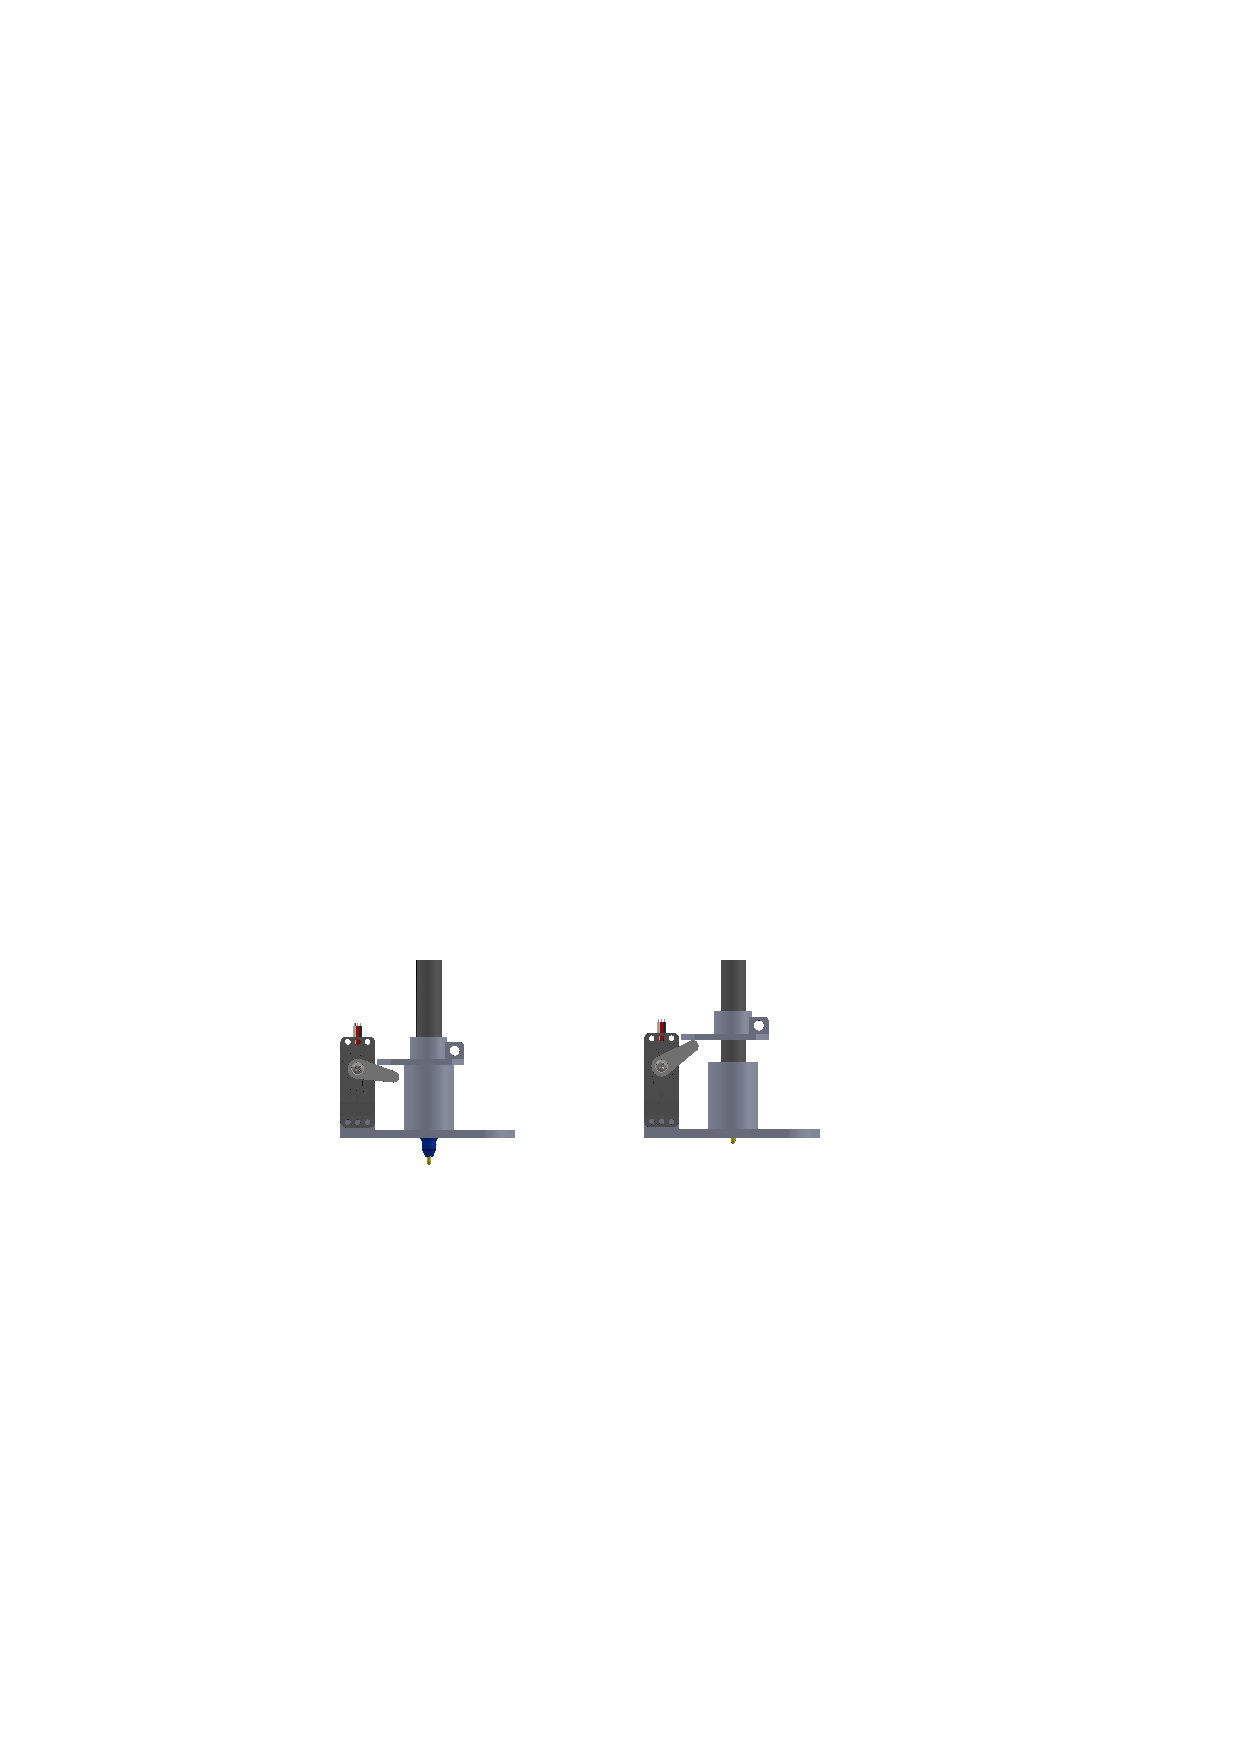
\includegraphics{GuiaServo}
	\caption{Servomotor muntat sobre la guia.}
	\label{fig:guiaservo}
\end{figure}


\section{Mecanisme d'elevació del retolador} \label{sec:suportmobil}

Aquest mecanisme consta d’una petita placa fixada a certa altura del retolador que actua com a superfície per tal de poder transformar el moviment circular del servo en el moviment vertical de l’utillatge. L’alçada a la qual s’ha de col·locar ve donada per la guia del retolador fixa al xassís (apartat \ref{sec:guia}), assegurant d'aquesta manera que quan el servomotor està en posició de dibuix aquest suport es recolzi a la cara plana superior de la guia i el retolador estigui en contacte amb el paper. 

S’ha dissenyat amb una part més allargada (detall 1 de la imatge \ref{fig:suport}) per tal d’assegurar el contacte i l’acció del servomotor al aixecar el braç, i a l'altre costat s’ha deixat un espai buit i dues parets verticals foradades (detall 2) per poder fixar l’estri amb l’ajuda d’un cargol un cop ajustada l'altura a la qual s'ha de fixar. Aquesta alçada s'ha d'ajustar mantenint el servo en posició activa, el retolador tocant al paper i el suport recolzat a la cara superior de la guia. L’eix vertical (detall 3) serveix per tal d’assegurar la perpendicularitat de l’estri amb la base del suport. 

\begin{figure}[H]
	\centering
	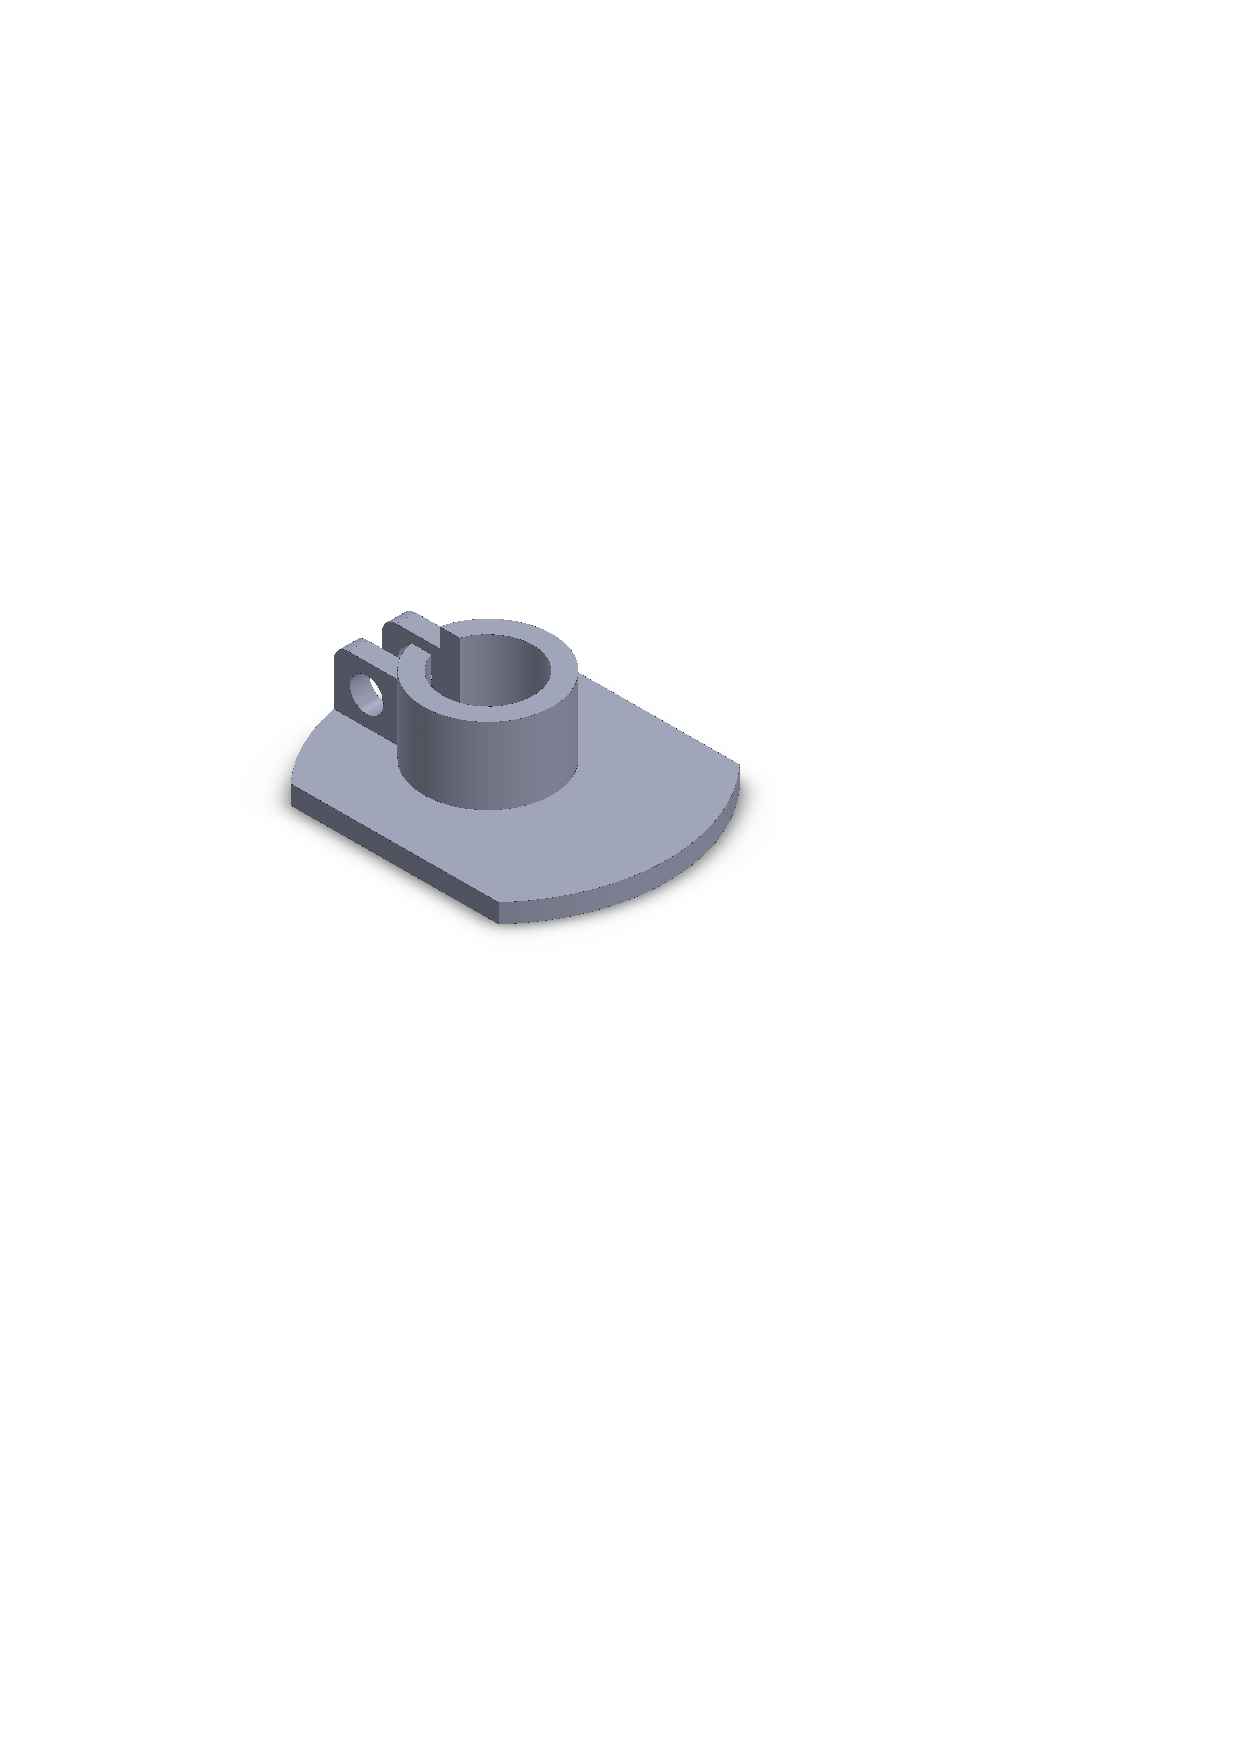
\includegraphics{suport}
	\caption{Imatge del disseny del suport pel mecanisme d'elevació.}
	\label{fig:suport}
\end{figure}

\section{Roda boja davantera}

Com a tercer punt de suport i per estabilitzar el robot, s’ha dissenyat una roda boja de manera que no intervingui en el moviment del robot, permetent el lliscament en qualsevol direcció. Consta de dues parts, el cos imprès en 3D i una bola de vidre que gira lliureament a l'interior. El cos assegura el contacte amb la bola en només 4 punts d’una circumferència paral·lela a la base fent així que el lliscament sigui més fàcil i minimitzant la força de fricció. També assegura que la bola es mantingui dins la cavitat quan s’aixeca el robot fet que provoca que la bola entri a pressió. La cara superior és una cara plana per facilitar la impressió 3D de la peça amb dos forats per fixar-la amb cargols al xassís i un forat per on es pot observar la bola per poder treure-la aplicant una petita pressió. 

\begin{figure}[H]
	\centering
	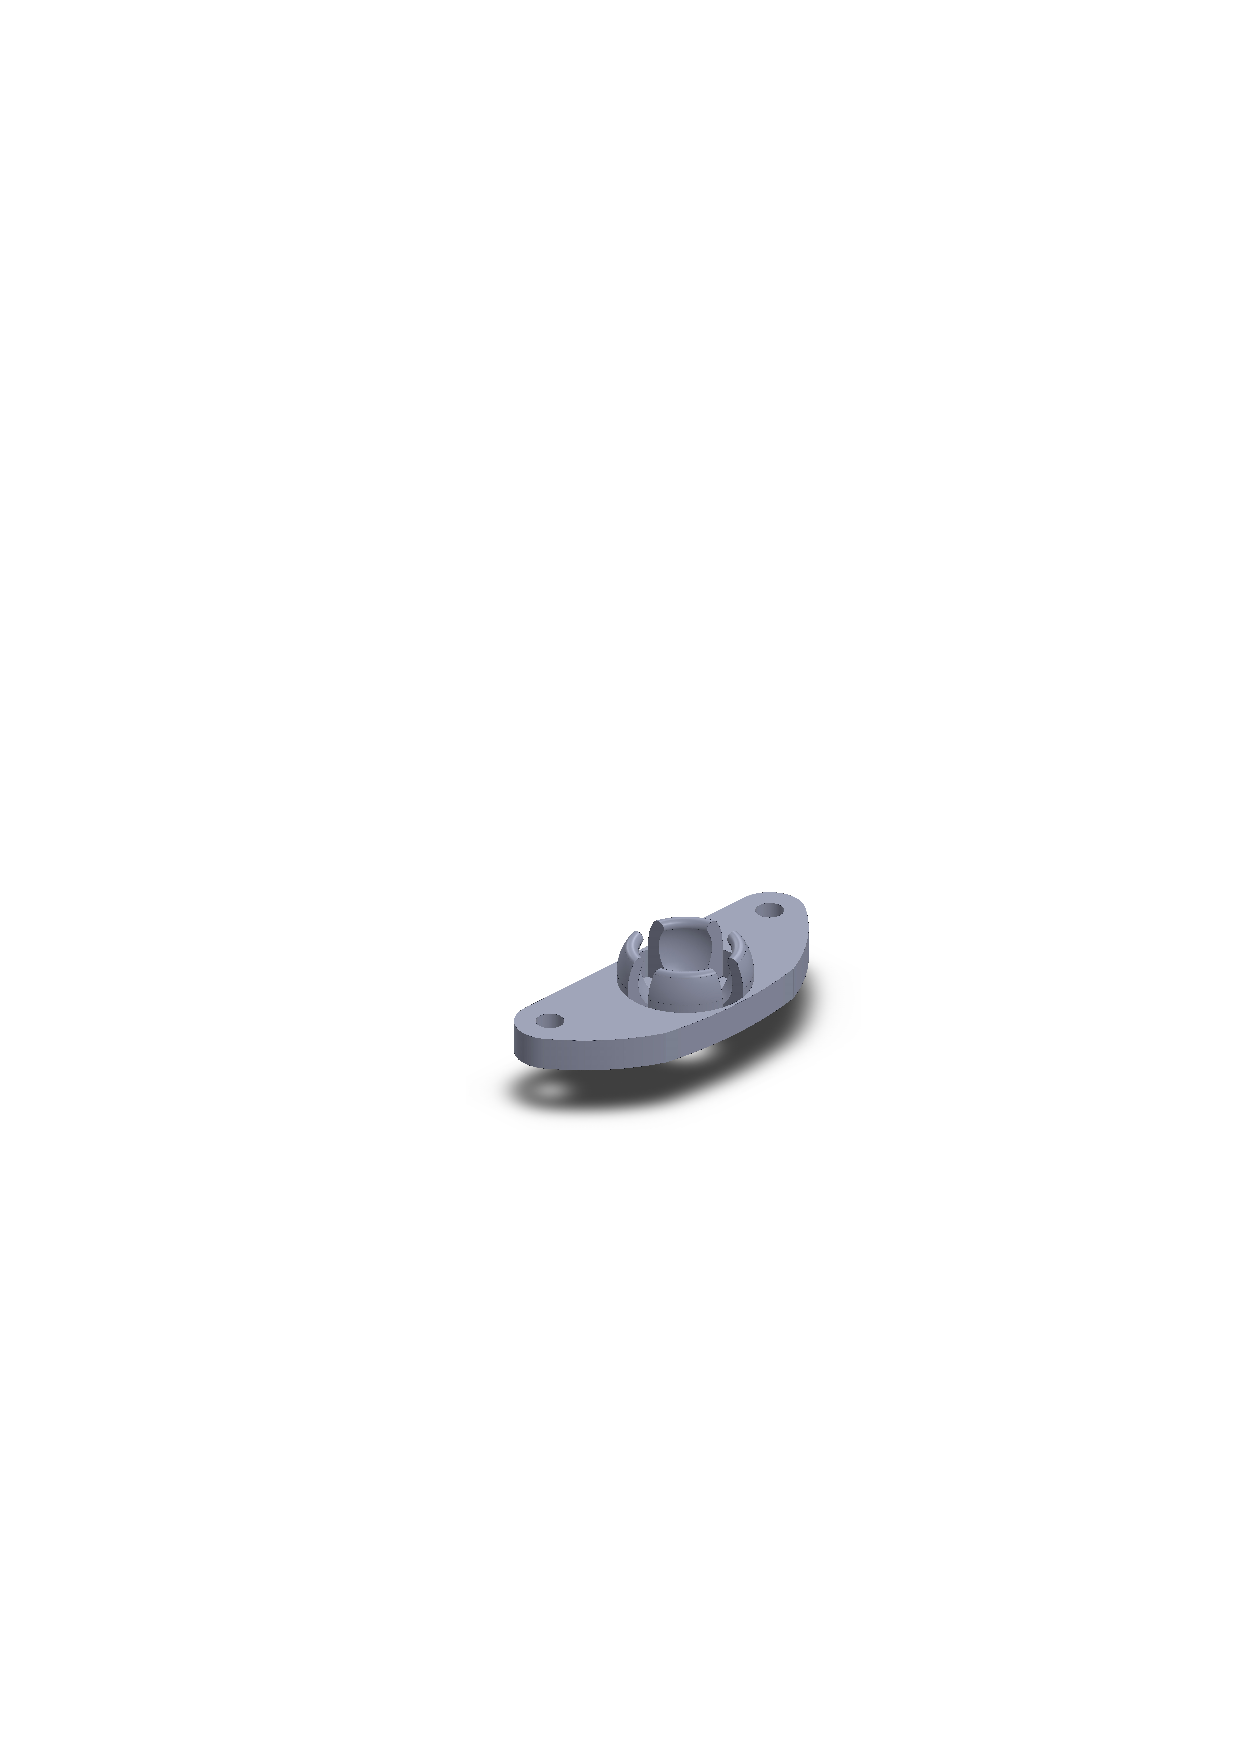
\includegraphics{bolaboja}
	\caption{Suport de la roda boja davantera.}
	\label{fig:bolaboja1}
\end{figure}

L’alçada de la roda, juntament amb les rodes motrius, són les encarregades de fixar l’alçada del robot, de manera que s’han dissenyat conjuntament per tal d’assegurar que la base sigui paral·lela al paper i mantenir l’eix del retolador vertical i centrat.

 \begin{figure}[H]
 	\centering
 	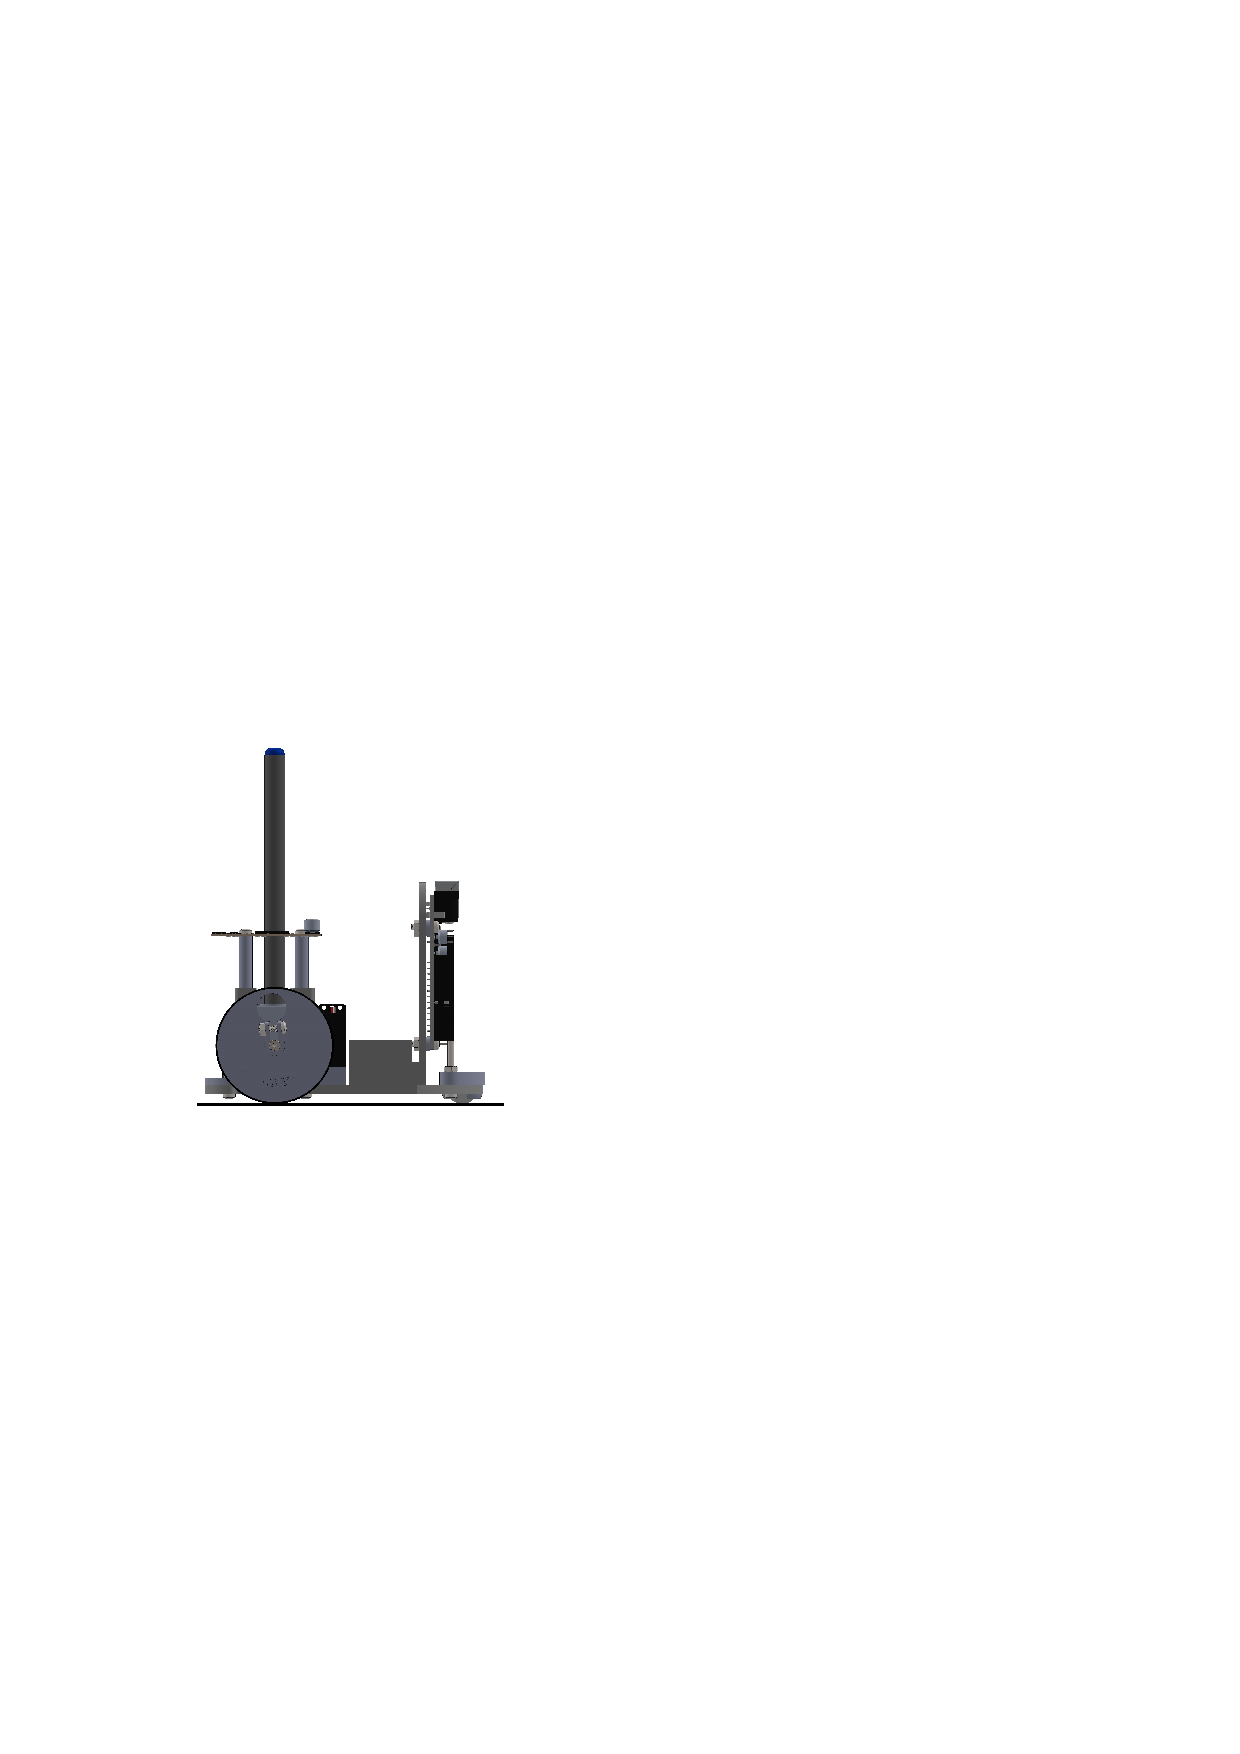
\includegraphics{pla}
 	\caption{Base del robot paral·lela al terra.}
 	\label{fig:pla}
 \end{figure}



\section{Rodes motrius}

Les rodes són una part fonamental del disseny, ja que són les encarregades del moviment del propi robot. Hi ha quatre aspectes bàsics per a la seva construcció: minimitzar la superfície de contacte amb el paper, assegurar la perpendicularitat i concentricitat amb l’eix, evitar el lliscament perquè giri de manera solidaria a l'eix i optimitzar el diàmetre per aconseguir un pas més precís disminuint al màxim el diàmetre. 

Per minimitzar la superfície de contacte amb el paper, s’ha decidit utilitzar una junta tòrica de goma d’1,5mm de diàmetre, que actua de la mateixa manera que els neumàtics d’un cotxe, evitant el lliscament amb el paper i, al ser circular, es minimitza el contacte fent-lo puntual o gairebé puntual. Així s’evita que un major contacte de la roda pugui actuar en contra del moviment del robot, creant forces de fricció que evitin la rotació del robot sobre el punt de contacte. Amb una superfície puntual també es millora la precisió dels moviments circulars, ja que es calculen a partir de la distància entre el retolador i la superfície de contacte i, per tant, com més petita sigui aquesta última, més exacta i constant serà aquesta distància durant el moviment radial de la roda. Per tal de mantenir el neumàtic a la roda, aquesta s’ha imprès directament amb un petit conducte amb la forma de mig neumàtic (detall 1 de la figura \ref{fig:roda}) aconseguint així que encaixin. 

En la pròpia impressió de la roda, s’ha afegit un eix transversal (detall 2) del mateix diàmetre que l’eix del motor per assegurar-ne d’aquesta manera la perpendicularitat i concentricitat. És un fet clau per assegurar el correcte funcionament, perquè, d’igual manera que al punt anterior, s’ha d’assegurar que la distancia entre les rodes sigui sempre la mateixa al llarg de tots els punts de la rotació de les mateixes, ja que és així com s’ha calculat la trajectòria. 

Un altre element del disseny són les dues petites parets verticals foradades (detall 3) que surten de l’eix i el forat que es pot observar al cos de la roda. Això permet que amb un cargol i una femella es pugui fixar la roda a l'eix, ja que es crea una deformació ínfima que redueix el forat a la mida exacte de l'eix del motor fent que quedin fixats sense alterar la forma de la roda. A  més, s'ha incorporat un forat a la pròpia roda (detall 4) que permet la manipulació dels cargols del motor sense la necessitat de treure la roda. 

Per acabar, el diàmetre de la roda s’ha intentat minimitzar de manera que es disminueix l’avanç de la roda per cada pas, augmentant així la precisió. Això s’ha realitzat tenint en compte la distància entre els eixos dels motors i la base, més una distància prudencial de 4,5 mm per poder col·locar els cargols necessaris per fixar els suports de l’utillatge de dibuix i la roda boja i mantenir-los separats del paper. D’aquesta manera s’han dissenyat unes rodes de 50,5 mm que sumat els neumàtics de goma acaba sent de 51,25 mm. 

\begin{figure}[H]
	\centering
	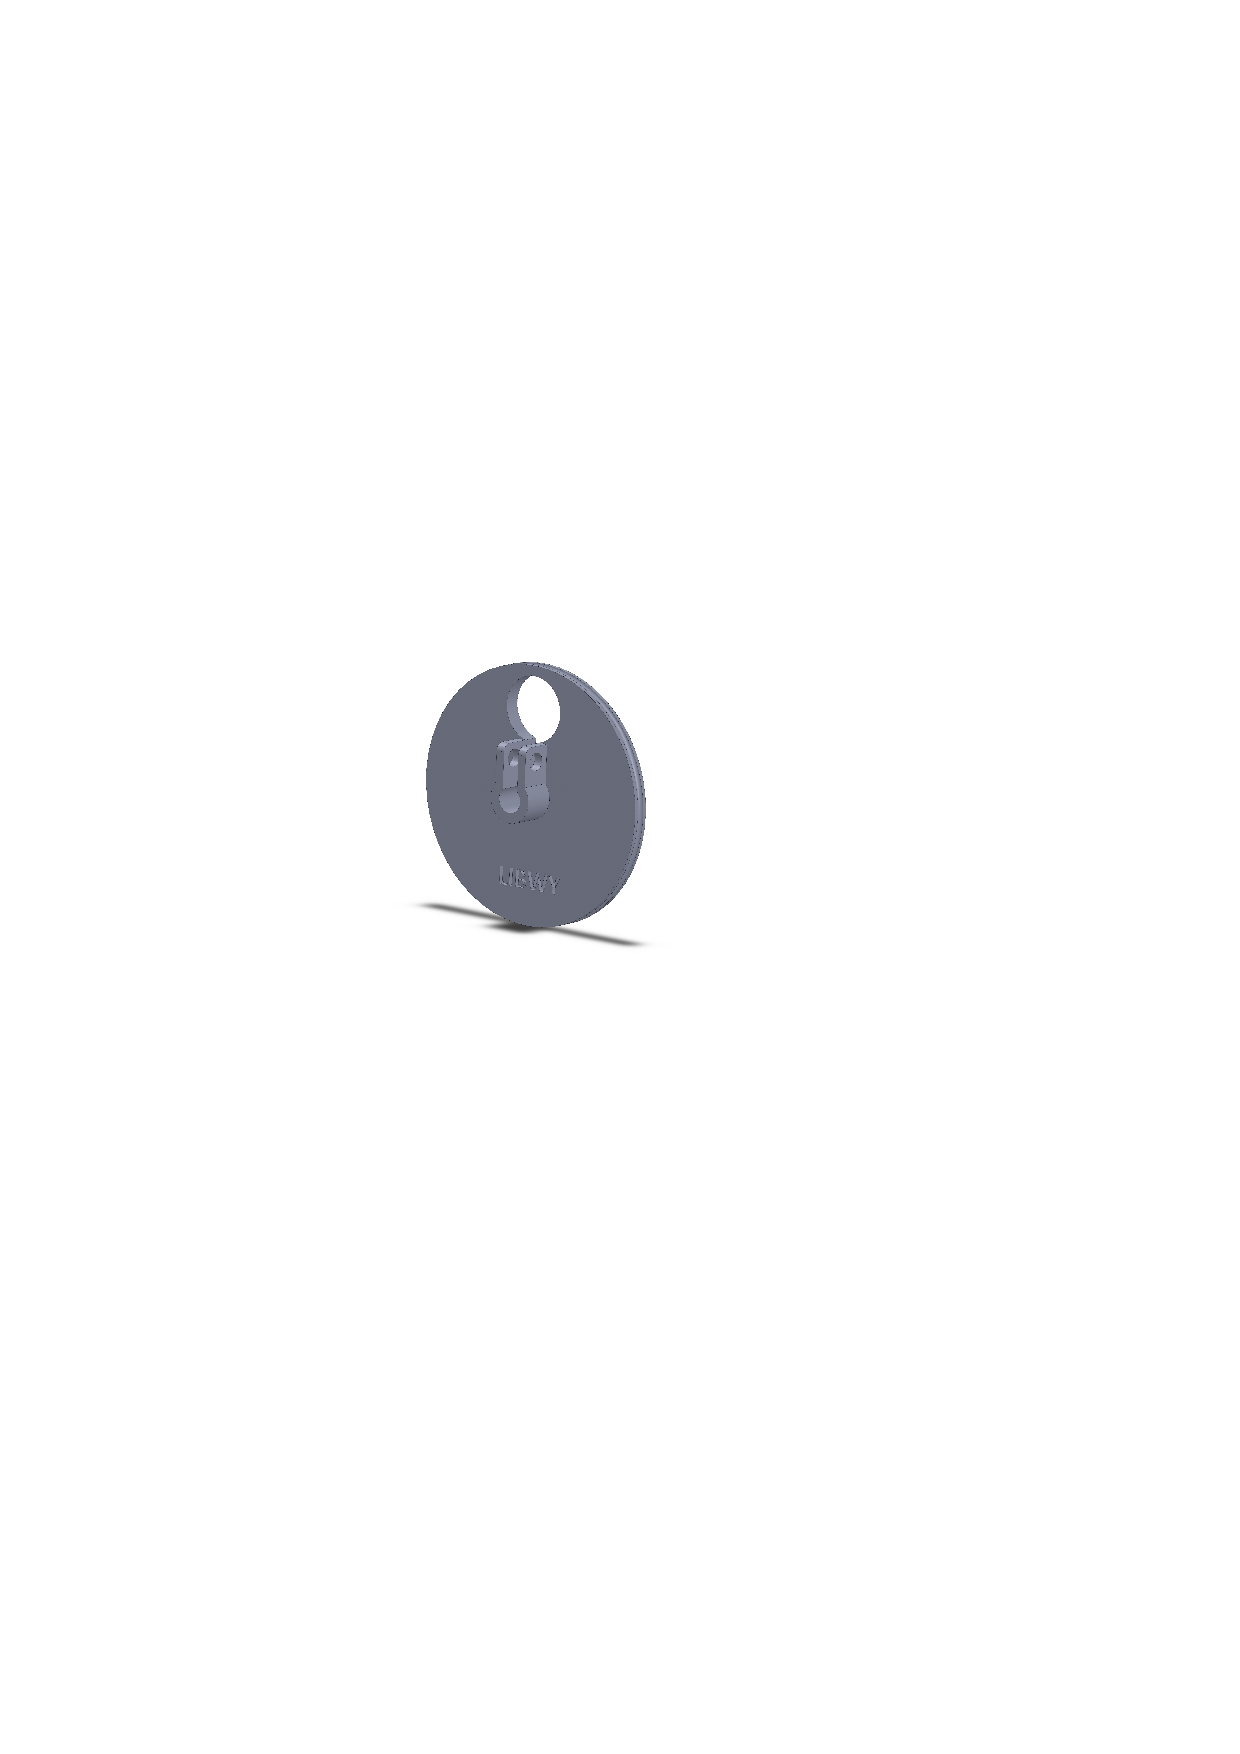
\includegraphics{roda}
	\caption{Disseny de la roda.}
	\label{fig:roda}
\end{figure}


\section{Cargols, femelles i tubs auxiliars}

Per l’assemblatge de tot el prototip s’han utilitzat cargols de mètrica M3 i les femelles adients per tal de fixar-los. S’han utilitzat un total de 14 cargols M3x10mm de llargada, 3 per fixar el suport del retolador, 3 per fixar la placa Arduino al xassís i 8 per fixar els motors als suports del xassís, 4 per cada motor. Per altre banda, s’han emprat 4 cargols M3x30mm per fixar els drivers (2 per cadascun) i 2 més per la roda boja davantera, que es podia fixar amb cargols més curts, però s’han utilitzat aquests per aprofitar els cargols disponibles. Tots els cargols porten una femella per tal de poder fer fixa la unió menys en el cas dels motors. En aquests, s'han utilitzat les femelles per escurçar la longitud del cargol i evitar el contacte amb els cargols posteriors del motor, ja que comparteixen eix. 

Per altra banda, s'han dissenyat i imprés en 3D uns tubs de plàstic, per tal d’elevar tant els drivers com la placa Arduino. En primer lloc, s’han aixecat els drivers 23 mm respecte els seus suports per permetre d’aquesta manera la correcta connexió dels cables, ja que aquesta connexió es realitza per la part inferior del mateix. Per altra banda, el microcontrolador s’ha separat 2 mm respecte la paret per així evitar el contacte dels pins soldats i evitar possibles sobreescalfaments. 

\begin{figure}[H]
	\centering
	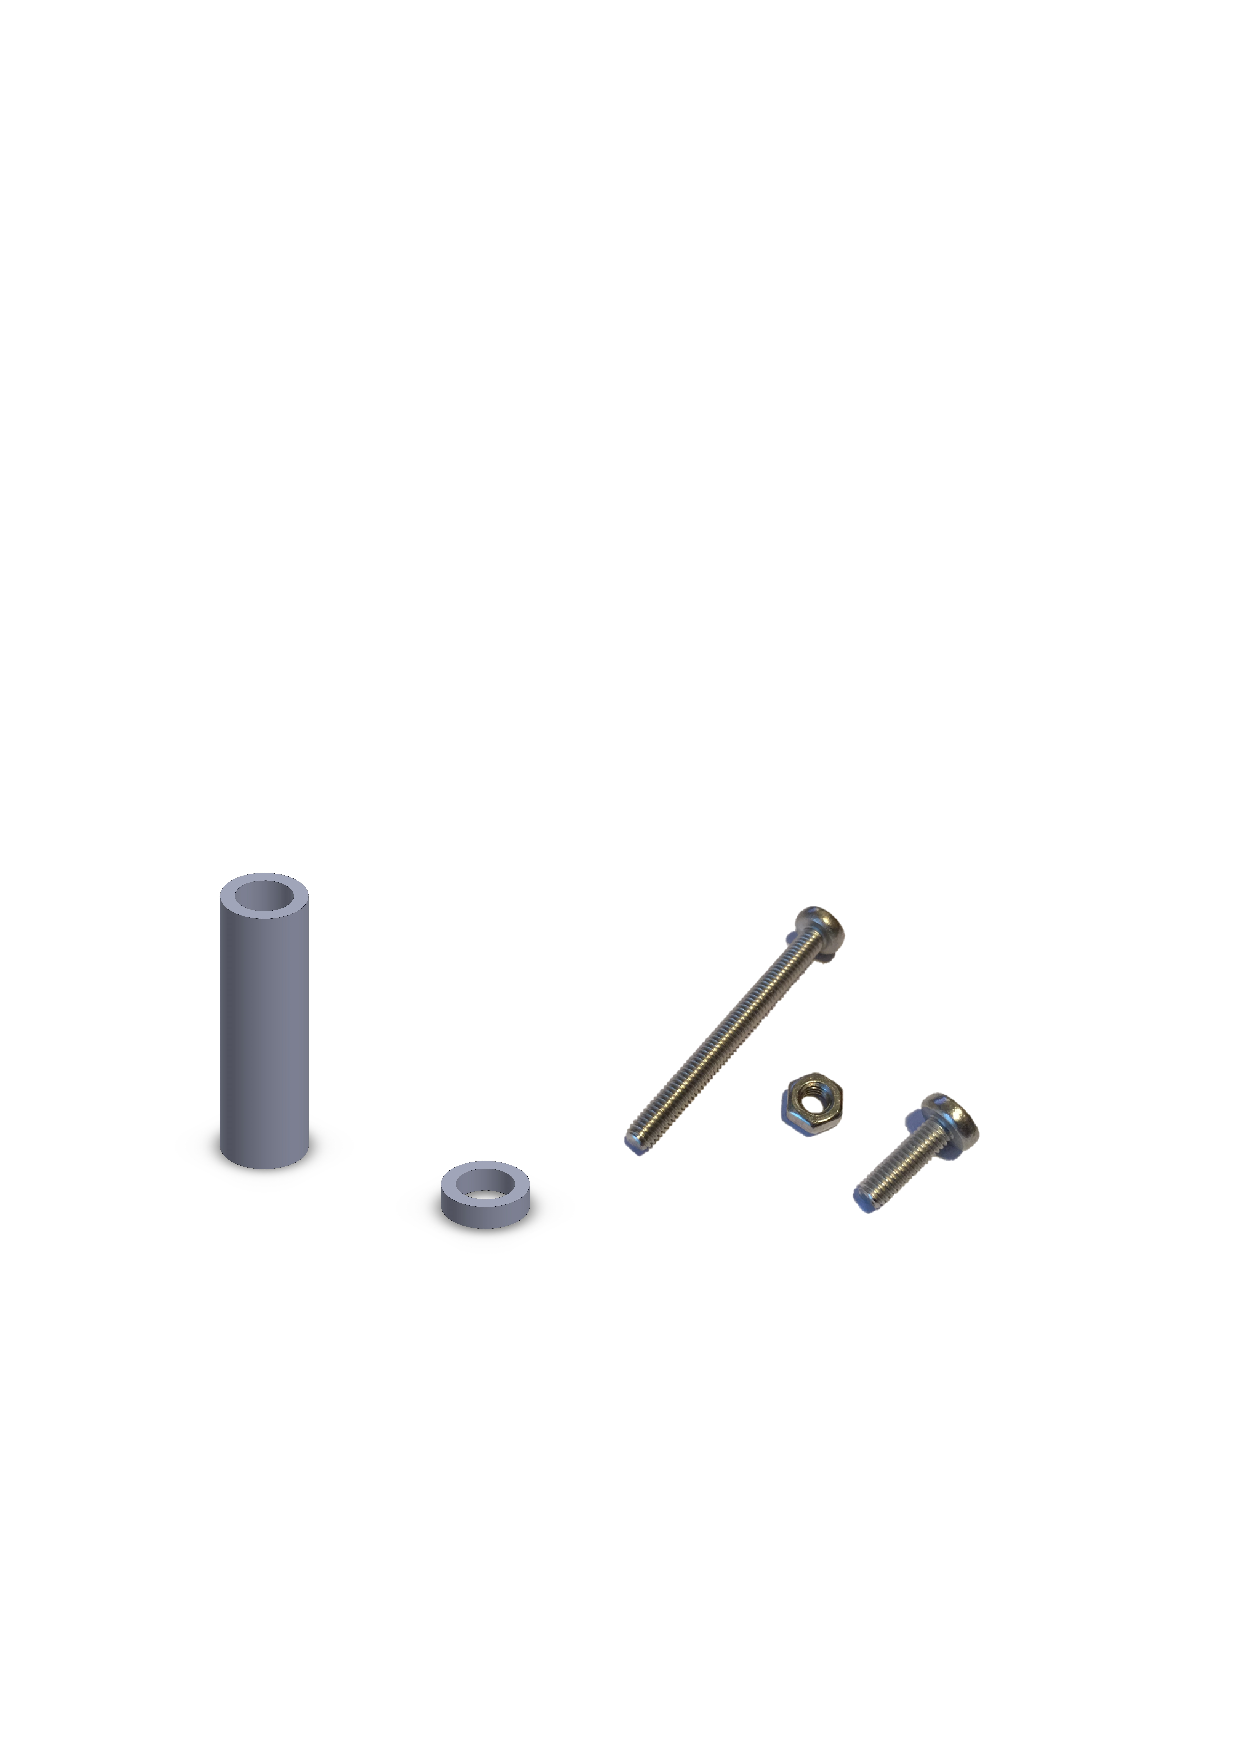
\includegraphics{tubs}
	\caption{Tubs auxiliars i exemples de cargols M3 i femelles utilitzats.}
	\label{fig:tubs}
\end{figure}
